\documentclass[]{llncs}
\title{A Formal Connection between Security Automata and JML Annotations
\thanks{This work is partially funded by the IST FET
programme of the European Commission, under the IST-2005-015905
\textsf{Mobius} project.}}

\author{Marieke Huisman\inst{1} \and Alejandro Tamalet\inst{2}\thanks{Research done while at INRIA Sophia Antipolis}}
\institute{INRIA Sophia Antipolis, France \and
University of Nijmegen, Netherlands}

\usepackage{amsmath}
\usepackage{amssymb}
\usepackage{bbold}
\usepackage{epsfig}
\pagestyle{plain}
\usepackage{xspace}
\newcommand{\PA}{\ensuremath{\mathit{PA}}\xspace}
\newcommand{\name}{\ensuremath{\mathsf{name}}\xspace}
\newcommand{\clname}{\ensuremath{\mathsf{clname}}\xspace}
\newcommand{\mname}{\ensuremath{\mathsf{mname}}\xspace}
\newcommand{\cps}{\ensuremath{\mathsf{cps}}\xspace}
\newcommand{\init}{\ensuremath{\mathsf{init}}\xspace}
\newcommand{\evs}{\ensuremath{\mathsf{events}}\xspace}
\newcommand{\vdsA}{\ensuremath{\mathsf{pa\_var\_decl}}\xspace}
\newcommand{\vdsP}{\ensuremath{\mathsf{prog\_var\_decl}}\xspace}
\newcommand{\trans}{\ensuremath{\mathsf{trans}}\xspace}

\newcommand{\setof}[1]{\ensuremath{\mathcal{P}(#1)}}
\newcommand{\CP}{\ensuremath{\mathit{CP}}\xspace}
\newcommand{\EVENT}{\ensuremath{\mathit{Event}}\xspace}
\newcommand{\VarDeclA}{\ensuremath{\mathit{PAVarDecl}}\xspace}
\newcommand{\VarDeclP}{\ensuremath{\mathit{ProgVarDecl}}\xspace}
\newcommand{\TRANS}{\ensuremath{\mathit{Trans}}\xspace}


\newcommand{\Name}{\ensuremath{\mathcal{N}}\xspace}
\newcommand{\type}{\ensuremath{\mathsf{type}}\xspace}
\newcommand{\Type}{\ensuremath{\mathcal{T}}\xspace}

\newcommand{\entry}{\ensuremath{\mathsf{entry}}\xspace}
\newcommand{\exit}{\ensuremath{\mathsf{exit}}\xspace}
\newcommand{\excexit}{\ensuremath{\mathsf{exc\_exit}}\xspace}
\newcommand{\etype}{\ensuremath{\mathsf{etype}}\xspace}


\newcommand{\Bool}{\ensuremath{\mathsf{Bool}}\xspace}
\newcommand{\Int}{\ensuremath{\mathsf{Int}}\xspace}
\newcommand{\Ref}{\ensuremath{\mathsf{Ref}}\xspace}
\newcommand{\Void}{\ensuremath{\mathsf{Void}}\xspace}

% \newcommand{\IntSet}{\ensuremath{\bbbz}\xspace}
\newcommand{\IntSet}{\ensuremath{\mathbb{Z}}\xspace}
\newcommand{\BoolSet}{\ensuremath{\mathbb{B}}\xspace}


\newcommand{\B}{\ensuremath{\mathsf{B}}\xspace}
\newcommand{\I}{\ensuremath{\mathsf{I}}\xspace}
\newcommand{\R}{\ensuremath{\mathsf{R}}\xspace}
\newcommand{\Null}{\ensuremath{\mathsf{Null}}\xspace}
%\newcommand{\One}{\ensuremath{\mathbb{1}}\xspace}
\newcommand{\One}{\ensuremath{\bbbone\xspace}}

\newcommand{\Val}{\ensuremath{\mathcal{V}}\xspace}

\newcommand{\opr}{\ensuremath{\texttt{[\#\:}}}
\newcommand{\clr}{\ensuremath{\ \texttt{\#]}}}
\newcommand{\opri}{\ensuremath{\texttt{(\#\:}}}
\newcommand{\clri}{\ensuremath{\ \texttt{\#)}}}

\newcommand{\chooseop}{{\ensuremath{\varepsilon}}} % choose operator

\newcommand{\scp}{\ensuremath{\mathsf{source}}\xspace}
\newcommand{\tcp}{\ensuremath{\mathsf{dest}}\xspace}
\newcommand{\cp}{\ensuremath{\mathsf{current}}\xspace}
\newcommand{\event}{\ensuremath{\mathsf{event}}\xspace}
\newcommand{\guard}{\ensuremath{\mathsf{guard}}\xspace}
\newcommand{\action}{\ensuremath{\mathsf{action}}\xspace}
\newcommand{\actskip}{\ensuremath{\epsilon}} % action skip

\newcommand{\target}{\ensuremath{\mathsf{target}}\xspace}
\newcommand{\expr}{\ensuremath{\mathsf{expr}}\xspace}

\newcommand{\listof}[1]{\ensuremath{\mathsf{list[}{#1}\mathsf{]}}\xspace}

\newcommand{\Store}{\ensuremath{\mathit{Store}}\xspace}
\newcommand{\Stmt}{\ensuremath{\mathit{Stmt}}\xspace}
\newcommand{\Expr}{\ensuremath{\mathit{Expr}}\xspace}

\newcommand{\Plus}{\ensuremath{\mathsf{Plus}}\xspace}
\newcommand{\EvalN}{\ensuremath{\mathsf{Var_{\mathbb{I}}}\xspace}}
\newcommand{\EvalB}{\ensuremath{\mathsf{Var_{\mathbb{B}}}\xspace}}
\newcommand{\EvalR}{\ensuremath{\mathsf{Var_{\mathbb{R}}}\xspace}}

\newcommand{\NumExpr}{\ensuremath{\mathit{NumExpr}}\xspace}
\newcommand{\BoolExpr}{\ensuremath{\mathit{BoolExpr}}\xspace}
\newcommand{\RefExpr}{\ensuremath{\mathit{RefExpr}}\xspace}

\newcommand{\ttt}{\ensuremath{\mathsf{true}}\xspace}
\newcommand{\fff}{\ensuremath{\mathsf{false}}\xspace}

\newcommand{\Not}{\ensuremath{\mathsf{Not}}\xspace}
\newcommand{\Conj}{\ensuremath{\mathsf{And}}\xspace}
\newcommand{\GT}{\ensuremath{\mathsf{GT}}\xspace}
\newcommand{\Eq}{\ensuremath{\mathsf{Eq}}\xspace}

\newcommand{\Assign}{\ensuremath{\mathsf{Assign}}\xspace}
\newcommand{\BExpr}{\ensuremath{\mathsf{BExpr}}\xspace}
\newcommand{\CondExpr}{\ensuremath{\mathsf{CondExpr}}\xspace}
\newcommand{\Call}{\ensuremath{\mathsf{Call}}\xspace}
\newcommand{\NExpr}{\ensuremath{\mathsf{NExpr}}\xspace}
\newcommand{\RExpr}{\ensuremath{\mathsf{RExpr}}\xspace}

\newcommand{\CaseJML}{\ensuremath{\mathsf{CaseSet}}\xspace}
\newcommand{\IfThenElse}{\ensuremath{\mathsf{IfThenElse}}\xspace}
\newcommand{\Sequence}{\ensuremath{\mathsf{Sequence}}\xspace}
\newcommand{\Set}{\ensuremath{\mathsf{Set}}\xspace}
\newcommand{\Skip}{\ensuremath{\mathsf{Skip}}\xspace}
\newcommand{\StmtExpr}{\ensuremath{\mathsf{StmtExpr}}\xspace}
\newcommand{\Throw}{\ensuremath{\mathsf{Throw}}\xspace}
\newcommand{\TryCatch}{\ensuremath{\mathsf{TryCatchFinally}}\xspace}
\newcommand{\While}{\ensuremath{\mathsf{While}}\xspace}
\newcommand{\Const}{\ensuremath{\mathsf{Const}}\xspace}
\newcommand{\Assert}{\ensuremath{\mathsf{Assert}}\xspace}

\newcommand{\Excpt}{\ensuremath{\mathcal{E}}}

\newcommand{\FieldDecl}{\ensuremath{\mathit{Decl}}\xspace}
\newcommand{\ArgDecl}{\ensuremath{\mathit{Decl}}\xspace}
\newcommand{\LocalVarDecl}{\ensuremath{\mathit{Decl}}\xspace}
\newcommand{\GhostVarDecl}{\ensuremath{\mathit{Decl}}\xspace}
\newcommand{\Decl}{\ensuremath{\mathit{Decl}}\xspace}


\newcommand{\Program}{\ensuremath{\mathit{Program}}\xspace}
\newcommand{\Class}{\ensuremath{\mathit{Class}}\xspace}
\newcommand{\Method}{\ensuremath{\mathit{Method}}\xspace}

\newcommand{\param}{\ensuremath{\mathsf{param}}\xspace}
\newcommand{\pre}{\ensuremath{\mathsf{pre}}\xspace}
\newcommand{\post}{\ensuremath{\mathsf{post}}\xspace}
\newcommand{\lvars}{\ensuremath{\mathsf{lvars}}\xspace}
\newcommand{\body}{\ensuremath{\mathsf{body}}\xspace}
\newcommand{\preset}{\ensuremath{\mathsf{pre\_set}}\xspace}
\newcommand{\postset}{\ensuremath{\mathsf{post\_set}}\xspace}
\newcommand{\excset}{\ensuremath{\mathsf{exc\_set}}\xspace}
\newcommand{\res}{\ensuremath{\mathsf{res}}\xspace}
\newcommand{\restype}{\ensuremath{\mathsf{res\_type}}\xspace}
\newcommand{\super}{\ensuremath{\mathsf{super}}\xspace}
\newcommand{\inv}{\ensuremath{\mathsf{inv}}\xspace}
\newcommand{\ghostvars}{\ensuremath{\mathsf{ghost\_vars}}\xspace}
\newcommand{\fields}{\ensuremath{\mathsf{fields}}\xspace}
\newcommand{\methods}{\ensuremath{\mathsf{methods}}\xspace}

\newcommand{\classes}{\ensuremath{\mathsf{classes}}\xspace}

\newcommand{\Pstate}{\ensuremath{\mathit{PState}}\xspace}
\newcommand{\FullProgram}{\ensuremath{\mathit{FullProgram}}\xspace}
\newcommand{\Mprogram}{\ensuremath{\mathit{MProgram}}\xspace}
\newcommand{\FullState}{\ensuremath{\mathit{FullState}}\xspace}
\newcommand{\Astate}{\ensuremath{\mathit{AState}}\xspace}
\newcommand{\Mstate}{\ensuremath{\mathit{MState}}\xspace}
\newcommand{\PAstate}{\ensuremath{\mathit{PAState}}\xspace}
\newcommand{\pstate}{\ensuremath{\mathsf{pstate}}\xspace}
\newcommand{\progstate}{\ensuremath{\mathsf{prog\_state}}\xspace}
\newcommand{\program}{\ensuremath{\mathsf{program}}\xspace}
\newcommand{\PStore}{\ensuremath{\mathit{PStore}}\xspace}
\newcommand{\pa}{\ensuremath{\mathsf{pa}}\xspace}
\newcommand{\pastate}{\ensuremath{\mathsf{pa\_state}}\xspace}
\newcommand{\ex}{\ensuremath{\mathsf{exc}}\xspace}
\newcommand{\st}{\ensuremath{\mathsf{store}}\xspace}
\newcommand{\stA}{\ensuremath{\mathsf{store_A}}\xspace}
\newcommand{\Excp}{\ensuremath{\mathit{Excp}}\xspace}
\newcommand{\Norm}{\ensuremath{\mathsf{Norm}}\xspace}
\newcommand{\Throwable}{\ensuremath{\mathsf{Throwable}}\xspace}
\newcommand{\NullPointer}{\ensuremath{\mathsf{RunTimeException}}\xspace}
\newcommand{\JMLExc}{\ensuremath{\mathsf{JMLException}}\xspace}
\newcommand{\fvs}{\ensuremath{\mathsf{fields}}\xspace}
\newcommand{\gvs}{\ensuremath{\mathsf{ghost\_vars}}\xspace}
\newcommand{\newgvs}{\ensuremath{\mathsf{new\_vars}}\xspace}
\newcommand{\unique}{\ensuremath{\mathsf{unique}}\xspace}
\newcommand{\lvs}{\ensuremath{\mathsf{loc\_vars}}\xspace}

\newcommand{\exc}{\ensuremath{\mathit{exc}}\xspace}
\newcommand{\act}{\ensuremath{\mathit{act}}\xspace}

\newcommand{\etp}[3]{%
  {#1} \vdash \langle {#2} \rangle \triangleright \langle {#3} \rangle}
\newcommand{\stp}[2]{%
  P \vdash \langle #1 \rangle \Rightarrow_P #2}

\newcommand{\gammain}{\ensuremath{\gamma_{\textsc{in}}}\xspace}
\newcommand{\gammanorm}{\ensuremath{\gamma_{\textsc{norm}}}\xspace}
\newcommand{\gammaexc}{\ensuremath{\gamma_{\textsc{exc}}}\xspace}
\newcommand{\gammapa}{\ensuremath{\gamma_{\textsc{pa}}}\xspace}

\newcommand{\deltaeval}{\ensuremath{\delta_{\textsc{eval}}}\xspace}
\newcommand{\deltaset}{\ensuremath{\delta_{\textsc{set}}}\xspace}
\newcommand{\deltacase}{\ensuremath{\delta_{\textsc{case}}}\xspace}
\newcommand{\deltaassert}{\ensuremath{\delta_{\textsc{assert}}}\xspace}

\newcommand{\md}{\ensuremath{\mathit{md}}\xspace}
\newcommand{\ev}{\ensuremath{\mathit{ev}}\xspace}
\newcommand{\invar}{\ensuremath{\mathit{inv}}\xspace}
\newcommand{\mn}{\ensuremath{\mathit{mn}}\xspace}
\newcommand{\with}{\ensuremath{\mathsf{\:with\:}}}
\newcommand{\id}{\ensuremath{\mathsf{id}}\xspace}


\newcommand{\br}[1]{\lbrack #1\rbrack}
\newcommand{\pif}[3]{\mathsf{if}\, #1\, \mathsf{then}\: #2\, \mathsf{else}\: #3}

\newcommand{\oldlvs}{\ensuremath{\mathit{old\_lvs}}\xspace}
\newcommand{\halted}{\ensuremath{\mathsf{halted}}\xspace}
\newcommand{\stuck}{\ensuremath{\mathsf{stuck}}\xspace}

\newcommand{\bp}{\ensuremath{\phantom{(}}}


\newcommand{\url}[1]{\texttt{#1}}

%\newcommand{\marginnote}[1]{\marginpar{#1}}
\newcommand{\marginnote}[1]{{\marginpar{\footnotesize\it #1}}}

\newcommand{\complete}{\ensuremath{\mathsf{complete}}\xspace}

\newcommand{\updatelvs}{\ensuremath{\mathsf{update\_lvs}}\xspace}
\newcommand{\lookupmthd}{\ensuremath{\mathsf{lookup\_mthd}}\xspace}
\newcommand{\lookupinv}{\ensuremath{\mathsf{lookup\_inv}}\xspace}

\newcommand{\exl}{\ensuremath{\mathsf{ok}}\xspace}
\newcommand{\resl}{\ensuremath{\mathsf{result}}\xspace}
\newcommand{\lookup}{\ensuremath{\mathsf{lookup}}\xspace}

\usepackage{paralist}

\begin{document}

\maketitle
\begin{abstract}
Security automata are a convenient way to describe security
policies. They are often used to monitor an application, and to
interrupt it as soon it violates the security policy. But such a
scenario is not always convenient, therefore, we consider the security
automata as specification only, and verify adherence to it
statically. To achieve this, we generate JML annotations that inline
the monitor in the application.

The translation from security automata to program annotations is
defined in several steps:
\begin{inparaenum}[(\itshape i\upshape)]
\item complete the security automata, adding a special trap
state that should not be reached (whereas partial automata, describing
only the allowed transitions are sufficient for monitoring);
\item generate special set-annotations at the level of method
specifications, capturing the behaviour of the security automata,
together with an invariant stating that the error state should not be
reached; and
\item inline the annotations into the method body.
\end{inparaenum}
An annotation propagation algorithm can then be used to generate
appropriate pre- and postconditions that are sufficient to guarantee
adherence to the annotations, and that can be verified statically.

We have developed a generic program semantics that is instantiated for
monitoring and run-time annotation checking. We prove that every
translation step preserves the program behaviour. In particular this
means that monitoring will not find a security violation iff run-time
annotation checking will not find any annotation violation (provided
that earlier existing annotations are not violated either).

Both program semantics, translation and correctness proofs are
formalised using the PVS theorem prover. The correctness proofs
revealed several subtleties that have to be considered in the
definition of the algorithm, and the program behaviour.
\end{abstract}


\section{Introduction}


Smart cards are trusted personal devices whose characteristics are
regulated by the ISO 7816 standard. As other trusted personal devices,
smartcards are designed to store and process confidential data, and
can act as tokens to provide users with a secure electronic
representation in a large network. They are widely deployed and used
in application areas such as mobile telecommunications, banking,
transportation, electronic identity, and digital rights management
(DRM). Further, they hold the promise to play a key role in the
e-society, especially as a means to guarantee users a personalized,
global, and secure access to applications and services.


The prominent role played by trusted personal devices in security
sensitive applications make them an ideal target for
attacks. Traditionally, the main concern with smartcards has been with
hardware attacks in which the attacker gains access to confidential
information or disturbs the functioning of the card through
observation (e.g. of power or electro-magnetic radiations) or invasion
(e.g. overriding sensors or attaching probes). This issue is studied in
Deliverable D8.1.

The trusted personal device remains a specific domain where post
issuance corrections are very expensive due to the deployment process
and the mass production. Furthermore, the emergence of new generation
trusted personal devices increasingly connected to networks and
providing execution support for complex programs and the prospect of
logical attacks has urged the trusted personal devices industry to
improve the quality of their software, as logical attacks are
potentially easier to launch than physical attacks (for example they
do not require physical access to the device, and are easier to
replicate from one device to the other), and may have a huge impact.
In particular, a malicious attacker spreading over the network and
disconnecting or disrupting devices massively could have deep consequences.

This deliverable reports on the development of methodologies and tools
that increase confidence in applications.  For concreteness, we focus 
on Java applications that can be executed on devices that embed Java
Virtual Machines (JVM) or their variants, in particular Java Card
Virtual Machines (JCVM). Java enabled devices are a natural choice for
formal methods because:
\begin{inparaenum}[i)]
\item they are widely deployed in the field;
\item they feature mechanisms that contribute to the security of the
platform and the applications that execute over it;
\item detailed informal specifications of the Java platform are publicly
available, and can be scrutinized.
\end{inparaenum}
However, it should be clear that the methods presented in this document
are relevant to other execution platforms for trusted personal devices.


\subsection{Security issues}
While the focus of the deliverable is on application validation,
security is a holistic property of a system, and formal techniques
must therefore be employed at different levels to provide strong
guarantees about the security of a TPD and its applications.
Essentially, the levels are: the hardware, platform, the libraries,
and the applications.

The need to consider security at those levels is illustrated for
example by the case study described on Page 55 in Deliverable D8.2,
which is concerned with secure platforms. The development of secure
API is discussed in Deliverables D7.1 and D7.2. As previously mentioned,
hardware security is discussed in Deliverable D8.1.


\paragraph*{Platform} The TPD security architecture guarantees that
downloaded applications are innocuous and comply with some basic
policies related to typing, initialization or access control. Such
basic policies are the cornerstones upon which the overall security of
the smartcard will rely. Therefore it is important to verify that the
security architecture does enforce these basic policies as
intended. Thus, an important application of formal methods to TPD
security is platform verification, which aims at providing an abstract
model of the Java platform and security architecture, and at proving
that the security functions play their expected role.

\paragraph*{Libraries} However, it is not sufficient to show that
security functions are correctly designed. In particular, one also has
to ensure that other components of the infrastructure, in particular
API, are correctly designed and implemented. For the purpose of this
deliverable, where the focus is on Java based TPD, the Java API and
the Global Platform API constitute two prominent components of the
infrastructure whose correct design is central to security. 


\paragraph*{Applications} 
Platform and libraries verification is a fundamental step towards
guaranteeing the security of smartcards, and a prerequisite for Common
Criteria evaluations at the highest levels. Nevertheless, the
guarantees offered by the Java security architecture are limited, and
further verifications must be performed to verify that applications
make a legitimate use of the infrastructure, and do not attempt any
hostile action.

Thus, application validation is another important application of
formal methods to TPD security. To date, testing campaigns remain the
primary means to ensure the quality of applications. However, testing
campaigns are expensive and only provide partial guarantees with
regard to the reliability of software. Therefore, it is important to
develop other advanced techniques for applet validation.

There are many facets to applet validation, each with its own
objectives and techniques:
\begin{itemize}
\item one can enhance existing security architectures to enforce
security properties not addressed by current architectures, in
particular confidentiality and availability.  Verification can be
performed by enhanced bytecode verification mechanisms;


\item one can abandon the realm of type systems and its associated
benefits and choose develop logical methods for specifying and
verifying either automatically or efficiently a specific class of
security properties. Verification can be performed by (possibly
efficient and hence incomplete) logic-based proof inference
mechanisms;




\item one can exploit the expressive power of logical methods to
require that applications, or at least sensitive fragments of
applications, are subjected to functional verification, i.e. to
verifications that establish their correctness in terms of
functionality as well as security.
\end{itemize}



\subsection{Logical verification of security properties using JML}
In order to provide precise analyzes with a limited overhead, we
advocate an integrated approach where validation techniques of
increasing strength are used, starting from automated techniques such
as testing and moving towards formal validation using a combination of
automated and interactive tools. In addition, we aim at overcoming the
difficulty of introducing formal techniques in industrial processes by
providing notations and tools hiding the mathematical formalisms and
by integrating formal techniques into classical developers environment
so as to allow users to benefit from formal techniques without having
to learn new formalisms and to become experts.

All the tools and results presented in this document were developed
with this goal in mind, notably the choice of JML as assertion
language and the development of JACK and its associated feature.
Using those techniques, Java developers should be able to validate
their code, or at least to get a good assurance on its correctness.


\subsubsection{JML}
JML~\cite{Leavens-Baker-Ruby99b,Leavens-Baker-Ruby03}, the ``Java
Modeling Language'', is a behavioral interface specification language
for Java; that is, it specifies both the behavior and the syntactic
interface of Java code.  The syntactic interface of a Java class or
interface consists of its method signatures, the names and types of
its fields, etc.  This is what is commonly meant by an application
programming interface (API).  The behavior of such an API can be
precisely documented in JML annotations; these describe the intended
way that programmers should use the API.  In terms of behavior, JML
can detail, for example, the preconditions and postconditions for
methods as well as class invariants. These specifications are given as
annotations of the Java source file. More precisely, they are included
as special Java comments, either after the symbols \lstinline!//@! or
enclosed between \lstinline!/*@! and
\lstinline[basicstyle=\normalfont\ttfamily\small\sl]!@*/!. For example,
the general schema for the annotation of a method is the following:
\begin{lstlisting}
/*@ behavior
  @   requires <precondition>;
  @   ensures <postcondition if no exception raised>;
  @   signals(E) <postcondition when exception E raised>;
  @   assignable <modified fields and variables>;
  @*/
\end{lstlisting}
where \lstinline!requires! specifies the conditions on variables, fields
and method parameters at the beginning of the method call so that the
conditions after \lstinline!ensures! hold at the end of the method
call and the conditions after \lstinline!signals(E)! hold if an
exception is raised and not caught inside the analyzed method.  The
underlying model is a an extension of Hoare-Floyd logic: if the
precondition holds at the beginning of the method call, then
postconditions (with and without exceptions) will hold after the
call. The \lstinline!assignable! clause specifies side-effect affected
variables and is used during the weakest precondition calculus for
method invocations.

An important goal for the design of JML is that it should be easily
understandable by Java programmers. This is achieved by staying as
close as possible to Java syntax and semantics.  Another important
design goal is that JML {\em not} impose any particular design method
on users; instead, JML should be able to document Java programs
designed in any manner \cite{Leavens-Baker-Ruby03}.

JML uses Java's expression syntax in assertions,
thus JML's notation is easy for programmers to learn.  
Because JML supports quantifiers such as
\verb_\forall_ and \verb_\exists_, and because JML allows ``model''
(i.e., specification-only) fields and methods, specifications can
easily be made precise and complete.
JML assertions are written as special
annotation comments in Java code,
so that they are ignored by Java compilers but can be used
by tools that support JML\@.  Within annotation comments JML extends the
Java syntax with several keywords.  It also extends Java's expression syntax with several
operators.
The central ingredients of a JML specification are preconditions
(given in {\tt requires} clauses), postconditions (given in {\tt
  ensures} clauses), and (class and interface) invariants.  These are
all expressed as boolean expressions in JML's extension to Java's
expression syntax.
In addition to ``normal'' postconditions, the language also supports
``exceptional'' postconditions, specified in {\tt signals} clauses.
These can be used to specify what must be true when a method throws an
exception. 

\paragraph*{Styles of specification}
Due to its expressiveness and versatility, the JML specification
language supports several styles of specifications; the choice of one
style of specification over the others depends on the purpose of the
verification effort. In a nutshell, one can either opt for lightweight
specifications in which one introduces enough annotations to reason
about some specific safety property, such as the absence of
exceptions, or heavyweight specifications where functional behavior is
considered. There is of course a great liberty in how \lq\lq
lightweight\rq\rq\ or \lq\lq heavyweight\rq\rq\ a specification should
be, and different styles can be used in different parts of an
application.

In addition, one may opt for defensive specifications, in which methods
are annotated with preconditions that prevent exceptions to occur, or
offensive specifications, which use appropriate clauses to specify 
exceptional postconditions.

\subsubsection{Verification techniques and tools}

JML specifications correctness can be verified either during runtime
or statically~\cite{BurdyCCEKLLP03}. To be verified during runtime, the
source code must have been compiled using \texttt{jmlc}, which is a
enhanced Java compiler for JML annotated code. This compiler adds to
the generated program assertions checking instructions corresponding
to the JML specifications of the program: preconditions, postconditions 
and loop or class invariants. An exception is raised during the execution 
if a JML condition fails. The JML runtime assertion checker can be used
for unit testing~\cite{CL02:ecoop}.


For the static verification of Java programs, several tools are
available using (variations of) JML as specification language. These
tools adopt different compromises between soundness and automation,
and thus it is useful to use them in combination, starting from
automatic but unsound tools, and pursuing with sound but interactive
tools.  Among these tools, ESC/Java2~\cite{CK04:cassis} offers the higher
level of automation as it does not require any user interaction and
relies on the Simplify automatic prover. It is particularly useful for
checking null pointers or array bounds limits; however it is unsound
and incomplete.

In order to further increase the level of reliability of applications,
we propose a methodology based on static verification using
JACK~\cite{BRL-JACK}, a tool that generates proof obligations that
can be discharged using proof assistants or automatic provers.


\subsection{Main contributions}
The work reported in this deliverable builds upon the JACK tool,
that was initially developed within Gemplus. The tool development
was transferred to INRIA at the beginning of the project, with
the objective to improve and increase its functionalities so as
to address the needs of INSPIRED. The main contributions of the
work carried within INSPIRED are:
\begin{itemize}
\item support for verifying high-level security properties
\item support for verifying bytecode programs
\item validation of the methodology for estimating resource
usage and optimizing code for low-footprint.
\end{itemize}
In order to carry the above tasks and evaluations, it has also
been necessary to make many improvements to the tool itself.
It is not in the scope of the present document to describe these 
improvements.


\subsection{Contents of the deliverable}
This document is organized as follows, the next chapter introduce the
assertion language JML, chapter 2 describes the JACK tool with its
extension feature, chapter 3 presents some evaluations done with the
tools and the last chapter concludes.

\section{Modelling Security Properties with Automata}\label{SecMVA}

This section formally defines the format of security automata that we
use. These are particularly suited for monitoring, because transitions
can depend on the state of the monitored program. We call them
Property Automata (PA).  
% \marginnote{MH: Multi-Variable Automata not very good/catchy name
%  AT: What about: Property Automata, Security Automata (or more precisely
%  Safety Automata), Pushdown Automata, just Automata or just Property.
%  I like Property Automata}
% \emph{Multi-Variable Automata} (MVA). %because their states are defined
%by a set of variables.
Transitions between states are labelled with guards, events and a list
of actions. The event specifies the method whose entry and/or exit is
being monitored, with a distinction between normal and exceptional
exits.  The guard describes the conditions under which the transition
can be applied. It depends on
\begin{inparaenum}[(\itshape i\upshape)]
\item the automaton state,
\item the state of the program that is being monitored, and
\item the argument of the method, in case the event is method entry;
the result of the method, in case the event is normal method exit; or
the exception with which the method returns, in case the event is
exceptional method exit.
\end{inparaenum}
Each action describes how the automaton state is updated by the transition.
% \marginnote{\small MH: conditions on guards/actions?
%  AT: I wouldn't mention them we have the specification for all the details.}

Throughout, we assume that \(\CP\) and \(\Name\) are infinite, but
enumerable nonempty sets of control points and names, respectively.
PA and programs share the definitions of values, types and exceptions,
denoted \Val, \Type and \Excpt, respectively. They are defined by the
following grammar, where \(\mathbb{B}\) and \(\mathbb{Z}\) denote the
standard sets of booleans and integers, respectively\footnote{We will
use a PVS-like notation to declare abstract data types and records
(enclosed by \(\opr\) and \(\clr\)). Further, if \(x\) is a record
with field \textsf{y}, we use \(x.\mathsf{y}\) to access field
\textsf{y}, and \(x \opri\mathsf{y} := z\clri\) to denote the record
\(x\) with the field \textsf{y} updated to \(z\).}.
\[{\small
\begin{array}{rcl}
\Val & = & \B(b : \mathbb{B}) \mid \I(i : \mathbb{Z}) \mid \Null \mid
\R(i : \mathbb{Z}) \mid \One \mid \bot\\
\Type & = & \Bool \mid \Int \mid \Ref \mid \Void\\
\Excpt & = & \Throwable \mid \NullPointer \mid \JMLExc
\end{array}}
\]
The special type \(\Void\), inhabited by \(\One\), models methods
without results. Reference values contain a number, which can be
considered as the location where the object is stored;
\(\bot\) is used to denote the outcome of an undefined expression.

% We assume that \(\Name\) contains the special names \textsf{this}.


A PA consists of
\begin{inparaenum}[(\itshape i\upshape)]
\item a name,
\item a class name, to specify which class is being monitored,
\item a finite set of control points,
\item an initial control point,
\item a set of events, to specify which methods are being monitored,
\item a set of PA variable declarations, to describe
the internal state of the automaton
\item a set of program variable declarations, to specify which
program variables will be inspected by the monitor, and
\item a set of transitions.
\end{inparaenum}
Transitions go from source to target control points. They are labelled
with events, where an event is a tuple of an event type (entry, exit
or exceptional exit) and a method name, guards and a list of
actions. Each action assigns the result of an expression (containing
both program and PA variables) to a PA
variable. Figure~\ref{FigPAForm} shows the main components of the
formal PA definition.

%  Variables
% declarations are the same as variable declarations in a program (defined
% below).
%  while program variable declarations in the PA have the same
% format as local variable declarations in a program (\emph{i.e.}, they
% are not explicitly initialised in the monitor, their value is retrieved from
% the program state.).
%% This is already said
% (the types of \FieldDecl and
% \LocalVarDecl will also be used in the abstract syntax of programs).

\begin{figure}[t]
\[{\small
\begin{array}{rcl}
\Decl & = \opr & \type : \Type, \name : \Name, \init : \Val
\clr \\
\EVENT & = \opr & \etype : (\entry \mid \exit \mid \excexit),
                 \mname : \Name \clr\\
\TRANS & = \opr & \scp, \tcp : \CP, \event : \EVENT, \action : (\opr \target : \Name, \expr : \Expr \clr)^*, \\
& &
\guard : \PAstate \times \Pstate \times (\Val \mid \Excpt) \rightarrow \mathbb{B}\clr\\
\PA & = \opr & \name, \clname : \Name, \cps : \setof{\CP},
            \init : \CP, \evs : \setof{\EVENT},\\
     &   &  \vdsA : \setof{\Decl}, \vdsP : \setof{\Decl},
            \trans : \setof{\TRANS} \clr
\end{array}}
\]
\caption{Formal Definition of PA}\label{FigPAForm}
\end{figure}

We require a PA to be \emph{deterministic}, \emph{i.e.}, for every
source control point and event there is always at most one guard that
holds. Notice that it is not obvious how to transform a
non-deterministic PA into a deterministic one, because the actions
made by the overlapping transitions might differ.
% We believe that this is a realistic restriction, and that most important
% security properties can be expressed as deterministic PAs.

A PA is \emph{total} if there is always a guard that holds
for a given source control point and event, otherwise it is
\emph{partial}. Every deterministic PA can be completed into a total
one (by function \complete): add a special control point
\halted, together with transitions for every control point and every event
to \halted, where the guard is the negation of the
disjunction of all other guards for this control point and event, and
in addition, add unconditional transitions from \halted to \halted
for every possible event.

%\marginnote{MH: Should we give formal definition of \emph{complete}?}

A PA is
\emph{wellformed} if\footnote{We only formalise constraints that are
necessary for our formalisation.}:
\begin{inparaenum}[(\itshape i\upshape)]
% \item the monitor variable names do not overlap with the reserved
% words,
% \item the program variable names that are used are unique,
\item variable names are unique and are not reserved words,
\item guards do not have side-effects,
\item guards and actions only use declared variables, and
\item control points and events  in transitions are declared.
% \item transitions range between declared control points and are
% labelled with declared events.
\end{inparaenum}

%Formally:
%\[
%\begin{array}[t]{l}
%\mathsf{complete}(a) =
%\begin{array}[t]{l}
%a \mathsf{with} (\#
%\begin{array}[t]{l}
%\cps := a.\cps \cup {\halted},
%\trans := a.\trans \cup complete(a.\trans)
%\end{array}
%\#)
%\end{array}
%\mathsf{complete}(T) =
%\{ (\# \scp := q,
%       \tcp := \halted,
%       \guard := \lambda \sigma_A \sigma_P v.
%\end{array}
%\]

% \paragraph{PA Transitions}
The state of a PA consists of a current control point, and the store of
automaton variables (the program store is not part of the automaton state).
\[{\small
\PAstate = \opr \cp : \CP, \stA : \Store \clr}
\]
Given PA \(a\), transition function \(\Delta_a\) specifies how an
automaton state \(\sigma_A\) is update, given program store
\(\sigma_P\) and event \(e\) (where \(\chooseop\) is the arbitrary
choice operator, and \textsf{apply} is a function that updates the
automaton store according to a list of actions in the obvious way).
\[{\small
\begin{array}{l}
\Delta_a  :  \PAstate \times \Pstate \times \EVENT \times (\Val \mid
\Excpt) \hookrightarrow
\PAstate\\
\Delta_a(\sigma_A, \sigma_P, e, v) = \\
\quad
\begin{array}[t]{l}
\mathsf{let\ }t = \chooseop(\{t\in \trans(a)\mid
  \begin{array}[t]{l}
     t.\scp = \sigma_A.\cp \wedge t.\event = e \wedge \\
     t.\guard(\sigma_A.\stA, \sigma_P.\fvs.\st, v)\}) \mathsf{\ in}
  \end{array}\\
\quad \opri \cp := t.\tcp, \stA := \mathsf{apply}(t.\action,
\sigma_A.\stA) \clri
\end{array}

\end{array}}
\]
In a total PA $a$, the transition function \(\Delta_a\) is total.
A partial automaton gets stuck on a certain input if and only if the
completed PA reaches the state \halted.

\begin{equation}\label{PAcompletionProp}
\Delta_a(\sigma_A, \sigma_P, e, v) = \perp \Leftrightarrow
\cp (\Delta_{\complete(a)}(\sigma_A, \sigma_P, e, v)) = \halted
\end{equation}


% The following PA\footnote{Where \(\actskip\) denotes an empty sequence.}
% encodes the property described in Figure~\ref{FigExample}.
% Recall the example security automaton in Figure~\ref{FigExample},
% expressing that the method \texttt{sendSMS} can
% be called at most \(N\) times in between calls to a \texttt{reset}
% method. This property is formally described by the following
% automaton\footnote{Where \(\actskip\) denotes an empty sequence.}.
% \[
% \small{
% \hspace{-0.3em}
% \begin{array}[t]{l}
% \opri
% \begin{array}[t]{l}
% \name := \textrm{LimitSMS}, \clname := \texttt{Messaging},
% \cps := \{s_1, s_2\},
% \init := s_1,\\
% \evs :=
% \begin{array}[t]{l}
% \{ \opri \etype := e, \mname := \texttt{sendSMS} \clri \mid e \in \opri \entry,
% \exit, \excexit \} \:\cup \\
% \{ \opri \etype := \exit, \mname := \texttt{reset} \clri\},
% \end{array}
% \\
% \vdsA := \{\opri \name := n, \type := \Int, \init := 0 \clri\},
% \vdsP := \emptyset,\\
% \trans := \{
% \begin{array}[t]{l}
% \opri
%  \begin{array}[t]{l}
% \scp := s_1, \tcp := s_2, \\
%              \event := \opri \etype := \entry,
%                              \mname := \texttt{sendSMS} \clri, \\
%              \guard := \lambda(\sigma_A, \sigma_P, v). n(\sigma_A) < N,
%              \action := \actskip
%             \clri,
% \end{array}\\
% \opri
%  \begin{array}[t]{l}
% \scp := s_2, \tcp := s_1, \\
%              \event := \opri \etype := \exit,
%                              \mname := \texttt{sendSMS} \clri, \\
%              \guard := \lambda(\sigma_A, \sigma_P, v). \ttt,
%              \action := [\opri \target := n, \expr := n + 1 \clri]
%             \clri,
% \end{array}\\
% \opri
%  \begin{array}[t]{l}
% \scp := s_2, \tcp := s_1, \\
%              \event := \opri \etype := \excexit,
%                              \mname := \texttt{sendSMS} \clri, \\
%              \guard := \lambda(\sigma_A, \sigma_P, v). \ttt,
%              \action := \actskip
%             \clri,
% \end{array}\\
% \opri
% \begin{array}[t]{l}
% \scp := s_1, \tcp := s_1, \\
%              \event := \opri \etype := \exit, \mname := \texttt{reset}
% \clri, \\
%              \guard := \lambda(\sigma_A, \sigma_P, v). \ttt,
%              \action := [\opri \target := n, \expr := 0 \clri]
%            \clri \} \clri
% \end{array}
% \end{array}
% \end{array}\\
% \end{array}
% }\]

\paragraph{Example}

The following PA\footnote{Where we assume that the default guard is
\(\lambda(\sigma_A, \sigma_P, v). \ttt\) and the default action is
\(\actskip\), an empty sequence.}
encodes the property described in Figure~\ref{FigExample}, while Figure~\ref{FigCompletePA} shows the completed PA.

\[
\small{
\hspace{-0.3em}
\begin{array}[t]{l}
\opri
\begin{array}[t]{l}
\name := \textrm{LimitSMS}, \clname := \texttt{Messaging},
\cps := \{s_1, s_2\},
\init := s_1,\\
\evs :=
\begin{array}[t]{l}
\{ \opri \etype := e, \mname := \texttt{sendSMS} \clri \mid e \in \opri \entry,
\exit, \excexit \} \:\cup \\
\{ \opri \etype := \exit, \mname := \texttt{reset} \clri\},
\end{array}
\\
\vdsA := \{\opri \name := n, \type := \Int, \init := 0 \clri\},
\vdsP := \emptyset,\\
\trans := \{
\begin{array}[t]{l}
\opri
 \begin{array}[t]{l}
\scp := s_1, \tcp := s_2, \guard := \lambda(\sigma_A, \sigma_P, v). n(\sigma_A) < N,\\
             \event := \opri \etype := \entry,
                             \mname := \texttt{sendSMS} \clri \clri,
\end{array}\\
\opri
 \begin{array}[t]{l}
\scp := s_2, \tcp := s_1, \action := [\opri \target := n, \expr := n + 1 \clri]\\
             \event := \opri \etype := \exit,
                             \mname := \texttt{sendSMS} \clri \clri,
\end{array}\\
\opri
 \begin{array}[t]{l}
\scp := s_2, \tcp := s_1, \\
             \event := \opri \etype := \excexit,
                             \mname := \texttt{sendSMS} \clri, \clri,
\end{array}\\
\opri
\begin{array}[t]{l}
\scp := s_1, \tcp := s_1, \action := [\opri \target := n, \expr := 0 \clri] \\
             \event := \opri \etype := \exit, \mname := \texttt{reset} \clri \clri
\} \clri
\end{array}
\end{array}
\end{array}\\
\end{array}
}\]


% Completion adds the following transitions to the automaton in
% Figure~\ref{FigExample}: from \(s_1\) to \halted, for the event
% \entry(\texttt{sendSMS}), with guard \(n \geq N\); and for the events
% \exit(\texttt{sendSMS}) and \excexit(\texttt{sendSMS}), with guard \ttt;
% from \(s_2\) to \halted, for the events \entry(\texttt{sendSMS}) and
% \exit(\texttt{reset}), with guard \ttt, from \halted to \halted, for
% all events and with guard \ttt.
% TODO AT: I get a reference to Figure 2 instead of 3. Moved label

\begin{figure}[t]

\psfrag{s1}{\tiny{\(s_1\)}}
\psfrag{s2}{\tiny{\(s_2\)}}
\psfrag{exit(sendSMS)?true -> n := n + 1;}
{\begin{tabular}{l}
\tiny{\exit(\texttt{SendSMS})?\ttt}\vspace*{-.8em}\\
\tiny{\(\rightarrow\)\texttt{n := n + 1};}
\end{tabular}}
\psfrag{exitE(sendSMS)?true -> ;}
{\begin{tabular}{l}
\tiny{\excexit(\texttt{sendSMS})?\ttt \(\rightarrow\)}%\vspace*{-.8em}\\
\tiny{\actskip;}
\end{tabular}}
\psfrag{exit(reset)?true -> n := 0;}
{\begin{tabular}{l}
\tiny{\exit(\texttt{reset})?\ttt \(\rightarrow\)}\vspace*{-.8em} \\
\tiny{\texttt{n :=} 0;}
\end{tabular}}
\psfrag{entry(sendSMS)? n<N -> ;}
{\begin{tabular}{l}
\tiny{\entry(\texttt{sendSMS})? \texttt{n} \(<\) \texttt{N} \(\rightarrow\)} %\vspace*{-.8em} \\
\tiny{\actskip;}
\end{tabular}}
\psfrag{entry(sendSMS)?true -> ;}
{\tiny{\entry(\texttt{sendSMS})?\ttt \(\rightarrow\)\actskip}}
\psfrag{exit(reset)?true -> ;}
{\tiny{\exit(\texttt{reset})?\ttt \(\rightarrow\)\actskip}}
\psfrag{exit(sendSMS)?true -> ;}
{\tiny{\exit(\texttt{sendSMS})?\ttt \(\rightarrow\)\actskip}}
\psfrag{exitE(sendSMS)?true -> ;}
{\tiny{\excexit(\texttt{sendSMS})?\ttt \(\rightarrow\)\actskip}}
\psfrag{entry(sendSMS)?n >= N -> ;}
{\tiny{\entry(\texttt{sendSMS})?\texttt{n} \(\geq\) \texttt{N}
\(\rightarrow\)\actskip}}
\psfrag{halted}{\tiny{\halted}}

\begin{center}
\epsfig{file=completed_alt.eps, width=7cm}
\end{center}
\caption{Automaton of Figure~\ref{FigExample}, after completion}\label{FigCompletePA}

\end{figure}



\section{Programs and Semantics}\label{SecProgram}

This section first defines an abstract syntax of programs, followed by
their semantics. Both are fairly standard, except that the semantics
is parametrised on the treatment of specifications. In particular, we
define a run-time checking and a monitoring semantics, that evaluate
differently upon method call and exit.


\subsection{Program Syntax}\label{SecSyntax}
Our language is a restricted subset of (sequential) Java, abstracting
away from typical object-oriented features, and in particular
from method resolution; instead we assume that
the annotated class contains method bodies for the relevant methods,
thus method lookup is trivial. We consider
only a few exceptions, and assume that methods have only one
parameter. We believe, however, that our formalisation contains all
constructs that are relevant for proving correctness of our inlining
algorithm for class-based monitoring, and implementing the
algorithm for the full language is mainly an engineering issue.

\begin{figure}[t]
\[{\small
\begin{array}{rcl}
\Expr & = & \Plus(n_1, n_2 : \Expr) \mid
            \EvalN(n : \Name) \mid
            \Not(b : \Expr) \mid
            \Conj(b_1, b_2 : \Expr) \mid \\
      &   & \Eq(e_1, e_2 : \Expr) \mid
            \EvalB(n : \Name) \mid
            \EvalR(n : \Name) \mid
            \CondExpr(c, e_1, e_2 : \Expr) \mid\\
      &   & \Assign(n : \Name, e : \Expr) \mid
            \Call(o : \Expr, mn : \Name, p : \Expr) \mid
            \Const(v : \Val) \\
\Stmt & = & \Skip \mid
            \Sequence(s_1, s_2 : \Stmt) \mid
            \IfThenElse(c : \Expr, s_1, s_2 : \Stmt) \mid\\
      &   & \While(c : \Expr, s : \Stmt) \mid
            \StmtExpr(e : \Expr) \mid
            \Throw(e : \Excpt) \mid\\
      &   & \TryCatch(t: \Stmt, e : \Excpt, c, f : \Stmt) \mid
            \Set(n : \Name, e : \Expr) \mid\\
      &   & \CaseJML(b : \listof{\Expr \times \Stmt}) \mid
            \Assert(e : \Expr)
\end{array}}
\]
\caption{Abstract syntax of expressions and statements}
\label{FigExprStmt}
\end{figure}

\begin{figure}[t]
\[{\small
\begin{array}{rcl}
\Method & = \opr & \name : \Name,
                   \param : \LocalVarDecl,
                   \lvars : \setof{\LocalVarDecl},
                   \body : \Stmt,\\
        &        & \res : \Expr,
                   \restype : \Type,
                   \pre, \post : \Expr \rightarrow \Expr, \\
        &        & \preset, \postset : \Expr \rightarrow \Stmt,
                   \excset : \Excpt \rightarrow \Stmt \clr \\
\Class & = \opr & \name : \Name,
                  \super : \Name_{\bot},
                  \fields : \setof{\FieldDecl},
                  \methods : \setof{\Method},\\
        &       & \inv : \Expr,
                  \ghostvars : \setof{\FieldDecl} \clr\\
\Program & = \opr & \classes : \setof{\Class} \clr
\end{array}}
\]
\caption{Abstract Syntax for Programs}\label{FigProgram}
\end{figure}


Figure~\ref{FigExprStmt} defines expressions and statements
% as a mutually recursive data type
(we use the term \emph{body} to denote either an expression or a
statement), \emph{e.g.}, \(\Call\) represents a call to method \(mn\) on
target \(o\) with argument \(p\). Notice that we define several
special language constructs to represent JML annotations: \Set, to
update ghost variables (\emph{i.e.}, specification-only variables),
\CaseJML, to abbreviate a list of conditional ghost variable updates,
and \Assert, to evaluate a condition on the program state. A standard
program semantics ignores these statements, whereas the annotated program
semantics evaluates them.

Figure~\ref{FigProgram} describes the syntax for methods,
classes and programs. To ensure that every method has an appropriate
return expression, it is part of the method signature.
Furthermore, methods can be annotated with pre- and postconditions, and
classes with invariants. To support our annotation generation
algorithm, we define special annotations called
\(\preset\), \(\postset\) and \(\excset\). These annotations describe
the updates to the ghost variables at method entry, exit and
exceptional exit, respectively.
Pre- and postcondition and the different method specification-level set
annotations have a function type to allow the use of the method parameter,
the method result, or the returned exception, respectively.

A program is said to be \emph{wellformed} if
\begin{inparaenum}[(\itshape i\upshape)]
\item names of fields, local variables and ghost variables are
disjoint and are not reserved words;
\item class names are unique;
\item method names are unique;
\item every variable name that is used is declared; and
\item only ghost variables are the target of \Set statements.
\end{inparaenum}
% (We have stated only the wellformedness conditions necessary for our
% correctness proofs.)


\subsection{Natural Semantics}\label{SecSemantics}
The behaviour of a program is described via a big step semantics. We
closely follow Von Oheimb's formalisation of Java~\cite{Oheimb01},
with simplifications wherever possible, due to our simplified
program syntax. A judgement $\etp{P}{e,\sigma}{v,\sigma'}$ means that the body
$e$ evaluates to $v$, while transforming the state $\sigma$ into $\sigma'$, in
the context of the program \(P\). Note that \(v\) is \One\ for
normally terminating \emph{statements}, while \(v\) is \(\bot\) whenever
evaluation finishes in an exceptional state.

A basic program state \(\Pstate\) is composed of an optional exception
and a store.  The store maps every field and local variable to a
value.

\[
{\small
\begin{array}{rcl}
\Pstate & = \opr & \ex : \Excp_{\bot}, \st : \PStore \clr\\
\PStore & = \opr & \fvs : \Name \mapsto \Val, \lvs : \Name \mapsto \Val \clr
\end{array}}
\]

Since annotated or monitored programs
contain more information than unannotated programs, the
evaluation rules are parametrised with types
\(\FullProgram\) and \(\FullState\). For each instantiation we give
mappings \program and \progstate to the basic program type \Program
and the basic program state \Pstate. Further, we add parameters that
specify the actions that are taken upon method entry or (normal or
exceptional) exit (\gammain, \gammanorm, and \gammaexc, respectively),
and the handling of annotations (\deltaset, \deltaassert, and
\deltacase).  In a standard program semantics, where specifications
are ignored, these are all instantiated with the identity relation.

The evaluation rules are fairly standard, and we refer to Von Oheimb
and the PVS formalisation for more details.  Evaluation
of normally terminating method calls is described by the following rule
(where for
clarity of presentation, we left out several checks that intermediate
states are not exceptional).

%\begin{figure}[t]
\vspace*{-1em}
\[{\small
\begin{array}{c}
\sigma_0.\progstate.\ex = \bot \qquad        % no exception in sigma_0
\etp{P}{o, \sigma_0}{r,\sigma_1} \qquad      % evaluate receiver
\etp{P}{p, \sigma1}{\act, \sigma_2}\\        % evaluate argument
%\sigma_2.\progstate.\ex = \bot \qquad        % no exceptions in sigma_2
r \not= \Null \qquad                         % receiver not null
\md = \lookupmthd(P, r, \mn) \\
\oldlvs = \sigma_2.\progstate.\st.\lvs \quad
\sigma_3 = \updatelvs(\sigma_2, r, \md.\lvars, md.\param, \act) \\
\gammain(P, \md, r, \Const(\act), \sigma_3, \sigma_4) \qquad
\etp{P}{\md.body, \sigma_4}{\One,\sigma_5} \\
\etp{P}{\md.\res, \sigma_5}{v,\sigma_6}\qquad
%\ex(\progstate(\sigma_6)) = \bot
\gammanorm(P, \md, r, \Const(v), \sigma_6, \sigma_7)\\
%\ex(\progstate(\sigma_7)) = \bot\\
\hline
\etp{P}{\Call(o,\mn,p), \sigma_0}{v, \sigma_7
(\progstate.\st.\lvs := \oldlvs)}
\end{array}}
\]
% \caption{Evaluation rule for normal termination of method
% calls}\label{FigEvalRules}
% \end{figure}

First the receiver is evaluated, resulting in non-null reference
\(r\).  Next, the parameter is evaluated, resulting in value
\act. Using \(r\), the method definition
\md is looked up.  The local variable store is updated assigning
\(r\) to \texttt{this}, initialising the method's local variables and
assigning the actual parameter to the formal parameter. The old local
variable store is remembered as \oldlvs.  Next, an appropriate action
upon method entry is taken, as specified by the relation
\(\gammain\). Then the method body, and method result expression are
evaluated. Since this rule applies to normal method termination only,
the parameter for normal method termination \(\gammanorm\) is
evaluated.  Last, the local store is set back to \(\oldlvs\). In
addition, rules exist that specify behaviour of a method call when it
is called upon a null reference, the body contains an uncaught
exception \emph{etc.}


\paragraph{Annotated Program Semantics}

The program state of an annotated program is extended with a store for
ghost variables:
\[{\small
\Astate = \opr \pstate : \Pstate, \gvs : \Name \mapsto \Val \clr}
\]
The types \FullProgram and \Program coincide, while \FullState is
instantiated as \Astate, and the mapping \progstate is defined as
\pstate. Figure~\ref{FigAnnotatedSem} shows some of the
instantiations of the semantics parameters; % (presented in rule format);
the other instantiations are similar. The relation \gammain
uses the auxiliary relation \(\beta\) which checks a boolean
expression \(e\) and raises a special \JMLExc if it evaluates to
false. Upon method entry, the class invariant and precondition are
evaluated. We assume that \(\lookupinv\) returns the complete class
invariant, including those invariants that are inherited from
superclasses.  If they fail, a \JMLExc is thrown, otherwise the
method's \preset statement is executed. Finally, we ensure that the
program store is not changed.  The function \deltaset updates a ghost
variable: it first evaluates the expression and if this did not result
in an exceptional state, it updates the value of the ghost
variable\footnote{Where \(\tau(\gvs.n := v)\) abbreviates that the
value of \(\gvs(n)\) in \(\tau\) is updated to
\(v\).} appropriately.

%% Relation with the code:
%% r = a, act = arg, \sigma_1 = s1, \sigma_2 = s2, \beta = check_assertion
\begin{figure}[t]
\[{\small
\begin{array}[t]{c}
\invar = \lookupinv(P, r) \qquad
\beta(P, \invar, \sigma_1, \tau_1) \qquad
\beta(P, \md.\pre(\act), \tau_1, \tau_2) \\
\etp{P}{md.\preset(\act), \tau_1}{v,\tau_2} \qquad v\in\{\bot,\One\} \qquad
\sigma_1.\pstate.\st = \sigma_2.\pstate.\st\\
\hline
\gammain(P, \md, r, \act, \sigma_1, \sigma_2)
\smallskip\\


\etp{P}{e, \sigma_1}{v, \tau} \qquad
\pif{v = \B(\ttt)}{\sigma_2 = \tau}{\sigma_2 = \tau (\ex := \JMLExc)}\\
\hline
\beta(P, e, \sigma_1, \sigma_2)

\smallskip\\

\etp{P}{e, \sigma_1}{v, \tau} \qquad
\pif{\tau.\pstate.\ex = \bot}{\sigma_2 = \tau (\gvs.n := v)}{\sigma_2 = \tau}\\
\hline
\deltaset(P, \Set(e, n), \sigma_1, \sigma_2)
\end{array}}
\]
\caption{Instantiation of semantics for runtime annotation evaluation}
\label{FigAnnotatedSem}
\end{figure}


\paragraph{Monitored Program Semantics}
The parametrised program semantics is also instantiated for monitored
programs. This semantics is only defined when the PA is compatible
with the program. PA \(a\) is said to be compatible with a program
\(P\), denoted \(a \sqsubseteq P\), if
\begin{inparaenum}[(\itshape i\upshape)]
\item the program contains the class \(c\) that is being monitored,
\item all variables declared as program variables in
\(a\) are fields of the class \(c\) with the correct type, and
\item every event name corresponds to a method in the class.
\end{inparaenum}
A monitored program is a product of a PA and a program. The state of a
monitored program consists of the states of the PA and the program
(including ghost variables)\footnote{For convenience, we assume that a
monitored program also evaluates annotations, but this instantiation
is in fact orthogonal to the annotated program semantics.}, and a flag
\stuck. If the PA is partial, the flag
\stuck is set when \(\Delta_a\) is not defined for a
certain input. If the flag is set, this means that the security policy
is violated, and the program should be stopped (by some external
observer). If the PA is total, the \stuck flag will never be
set. Instead, violation of the security policy is modelled by the PA
reaching the trap state \halted (in which case the external observer
again is supposed to stop execution).

\vspace*{-1em}
\[
{\small
\begin{array}{rcl}
\Mprogram & =  & \opr \pa : \PA, \program : \Program \clr\\
\Mstate & = & \opr \pastate : \PAstate, \pstate : \Pstate, \gvs :  \Name \mapsto \Val, \stuck
: \BoolSet \clr
\end{array}}
\]
Thus, \FullProgram gets instantiated as \Mprogram and \FullState as
\Mstate, with mappings \program and \pstate. Now we can give
appropriate instantiations for the \(\gamma\)- and
\(\delta\)-relations. The \(\delta\)-relations are the same as
for the annotated program semantics, but the \(\gamma\)-relation also
updates the state of the monitor. For example, \(\gammain\) is defined
in terms of \(\gammain\) for annotated programs, as defined in
Fig.~\ref{FigAnnotatedSem}.
\[
{\small
\begin{array}{c}
\gammain^{\mathsf{AP}}(P, \md, r, \act, \sigma_1, \tau) \\
\pif{\tau.\pstate.\ex = \bot}
    {\sigma_2 = \gammapa(\entry)(P, \md, \act, \tau)}
    {\sigma_2 = \tau}\\
\hline
\gammain(P, \md, r, \act, \sigma_1, \sigma_2)
\end{array}}
\]


\noindent where
% NOTE: This is a simplified version of on_method_MVA in MonitoredProgram
\[
{\small
\begin{array}[t]{rcl}
\gammapa(\ev)(P, \md, \act, \sigma) & = &
\begin{array}[t]{l}
\mathsf{let\ }
\begin{array}[t]{rcl}
  e & = & \opri \etype := \ev, \mname := \md.\name \clri,\\
 \tau & = & \Delta_{P.\pa}(\sigma.\pastate, \sigma.\progstate, e, \act)
\mathsf{\ in\ }\end{array}
\\
\pif{\sigma.\stuck \vee \tau = \bot}
    {\sigma (\stuck := \ttt)}
    {\sigma (\pastate := \tau)}
\end{array}
\end{array}}
\]

\section{Annotation Generation}\label{SecAnnotGen}

Given a security property encoded as an MVA, the annotation generation
procedure generates JML-annotations that capture this property,
\emph{i.e.}, if the program does not violate the generated
JML-annotations, it respects the security property encoded by the
MVA. As explained above, the procedure is defined in several steps:
\begin{inparaenum}[(\itshape i\upshape)]
\item the monitor is completed (as described in Section~\ref{SecMVA});
\item the annotations are generated at the method specification level,
as special set-annotations;
\item the method specification-level set-annotations are inlined in
the method body; and
\item the special \CaseJML construct that is used to make the
annotations more compact is translated into a sequence of \Set
annotations.
\end{inparaenum}
Notice that the order of the last two steps can be swapped.

For each step we basically prove that the old and the new program are
bisimilar, \emph{i.e.}, we show for every program translation step
\(\alpha\) there exists a relation \(R\) such that:
\[
\begin{array}{l}
\etp{P}{b,\sigma_1}{v_1, \sigma_2} \Rightarrow
\etp{\alpha(P)}{b, \tau_1}{v_2, \tau_2} \Rightarrow
R(\sigma_1, \tau_1) \Rightarrow
R(\sigma_2, \tau_2)
\end{array}
\]
If we then show that the initial program states are related by this
relation, we can conclude that any reachable states in the program are
related.

A natural way to prove this is by induction over the derivation
length. However, to be able to prove that this way, we have to make
some restrictions. In particular, many translation steps introduce new
(ghost) variables to encode the MVA. Therefore, to be able to apply
induction, we typically require that the body \(b\) does not contain
any new variables. The new variables occur only at specific points in
the program, and for these point separate preservation lemmas have to
be proven. Further, to be able to complete the proof, we need to
ensure that in both bodies the same branches of conditional
expressions and statements are taken, and that the same values get
assigned to the store. Therefore, we also prove that the resulting
values \(v_1\) and \(v_2\) are the same (however, sometimes this holds
only under certain conditions).



This section presents more details of the different translation steps,
and shows the relation that relates the derivations in the two
different programs. Further, for every step we discuss the conditions
under which the equivalence holds.

%\begin{figure}
%\begin{center}
%\epsfig{file=annotgen_example, width=4cm}
%\end{center}
%\caption{MVA fragment to illustrate set-annotation
%generation}\label{FigAnnotGenExample}

%\end{figure}

\paragraph{Completion of the automaton}
The first translation step does not change the program itself, it only
completes the MVA. Suppose that \(P\) is a monitored program, where
\(\mva(P)\) is deterministic and wellformed. Then the translation to a
monitored program with a total MVA, \(\alpha_1(P)\) is defined as:
\[
\opri \mva := \complete(\mva(P)), \program(P) \clri
\]

The relation that is preserved between executions of \(P\) and
\(\alpha_1(P)\) is the following (where \(\sigma\) is a state of
\(P\) and \(\tau\) is a state of \(\alpha_1(P)\)
\[R(\sigma, \tau) \hat=
 \begin{array}[t]{l}
  (\sigma.stuck \Leftrightarrow \tau.\mvastate.\cp = \halted) \:\wedge \\
  (\sigma.\mvastate.\stA = \tau.\mvastate.\stA) \:\wedge \\
  (\sigma.\progstate = \tau.\progstate)
\end{array}
\]

To prove that this relation is preserved for any body \(b\), we make
use of equivalence (\ref{MVAcompletionProp}) on
Page~\pageref{MVAcompletionProp} and we observe further that
\begin{inparaenum}[(\itshape i\upshape)]
\item if \stuck has been set, it remains set,
\item if \halted is reached, it is never left, and
\item if the MVA is total, \stuck is never set.
\end{inparaenum}. Formally, where \(P\) is a monitored program, and
\(Q\) is a monitored program with compete MVA:
\[
\begin{array}[t]{rl}
\sigma_1.\stuck \Rightarrow
\etp{P}{b,\sigma_1}{v,\sigma_2} \Rightarrow &
\sigma_2.\stuck \\
\sigma_1.\mvastate.\cp = \halted \Rightarrow
\etp{P}{b,\sigma_1}{v,\sigma_2} \Rightarrow &
\sigma_2.\mvastate.\cp = \halted \\
\neg \sigma_1.\stuck \Rightarrow
\etp{Q}{b,\sigma_1}{v,\sigma_2} \Rightarrow &
\neg \sigma_2.\stuck
\end{array}
\]

For our running example, applying translation \(\alpha_1\) means that
where class \texttt{Messaging} in Figure~\ref{FigExampleImplem} was
first monitored with the partial MVA in Figure~\ref{FigExample}, after
the translation it is monitored with the complete MVA in
Figure~\ref{FigCompleteMVA}.

\paragraph{From MVA to Annotations}

\begin{figure}[t]
\[
\begin{array}{rcl}
\alpha_2(P) & = &\opri \classes :=
\{\alpha_{2, \mathcal{C}}(c, \mva(P)) \mid c \in P.\classes\} \clri\\

\alpha_{2,\mathcal{C}}(c, a) & = &
\mathsf{if\ }c.\name = a.\clname\\
&&
\mathsf{then\ }c \:\opri
 \begin{array}[t]{l}
 \gvs := \gvs(c) \cup \newgvs(a)\\
 \inv := \Conj(\Not(\Eq(\texttt{cp}, \texttt{halted})), c.\inv)\\
 \methods := \{\alpha_{2,\mathcal{M}}(m, a) \mid m \in c.\methods\} \clri
\end{array}\\
&& \mathsf{else }c\\
\alpha_{2,\mathcal{M}}(m, a) & = & m \: \opri
  \begin{array}[t]{l}
  \preset := \begin{array}[t]{l}
             \preset(m); \alpha_{2,\mathcal{E}}(\entry, m.\name, a);\\
             \Assert(\Not(\Eq(\texttt{cp}, \texttt{halted}))),
             \end{array}\\
  \postset := \postset(m); \alpha_{2, \mathcal{E}}(\exit, m.\name, a)\\
  \excset := \excset(m); \alpha_{2, \mathcal{E}}(\excexit, m.\name, a)
  \clri
  \end{array}\\
\alpha_{2, \mathcal{E}}(e, n, a) & = &
  \alpha_{2, \mathcal{T}}(\{t \mid t \in a.\trans \wedge
                                   t.\event = \opri \event := e,
                                                    \mname := m \clri
                           \})\\
\alpha_{2, \mathcal{T}}(ts) & = &
  \CaseJML(
    \{(\begin{array}[t]{l}
       \Eq(\texttt{cp}, \texttt{q}),\\
       \CaseJML(\{(t.\guard, \Set(\texttt{cp}, t.\tcp; t.\action)) \mid
                  t \in ts \wedge t.\scp = \texttt{q}
               \}))\\
    \mid \texttt{q} \in a.\cps
    \})
    \end{array}
\end{array}
\]
\caption{Formal definition of translation MVA into annotations}
\label{FigMVAtoAnnot}
\end{figure}


Figure~\ref{FigMVAtoAnnot} contains the formal definition of the
second translation step: from MVA to method-level
set-annotations. Given a monitored program \(P\) where \(\mva(P)\) is
total. The annotation generation algorithm \(\alpha_2\) applies
\(\alpha_{2, \mathcal{C}}\) to all
class. This function checks whether the class is the one being
monitored. If so, appropriate ghost variables are added to the class
using function \newgvs, that is not formally defined here. Basically
\begin{inparaenum}[(\itshape i\upshape)]
\item for each control point of the automaton, a (final) ghost
variable declaration is generated, initialised to a unique value
(\emph{i.e.}, we assume we have a function \unique that maps each
control point to a unique value);
\item a ghost variable \texttt{cp} is declared, initialised to the
value of the ghost variable representing the initial control point;
\item for each automaton variable declaration, a ghost variable is
declared with corresponding type and initialisation.
\end{inparaenum}
Further, \(\alpha_{2, \mathcal{C}}\) adds the condition that the
current control point should not be halted to the class
invariant\footnote{For readability, we do not explicitly write the
translation from MVA control points to ghost variables.}, and then it
annotates all methods in the class using \(\alpha_{2,
\mathcal{M}}\). For each method in the class, its \preset, \postset
and \excset are extended with updates to the ghost variables encoding
the automaton. In addition, at the end of the \preset, an \Assert
statement is added to verify that the transition did not reach the
\halted state: in that case program execution should terminate
immediately, and without this \Assert, the invariant violation will
only be detected after the body is executed. To encode the updates to
the ghost variables, first \(\alpha_{2, \mathcal{E}}\) computes the
set of relevant transitions (\emph{i.e.}, those where the event and
method name correspond). For these transitions, a \CaseJML
statement is generated, where the different cases correspond to the current
control point being equal to a control point \texttt{q}, for any
\texttt{q} in the automaton. For each such \texttt{q}, all transitions
with \(t.\scp\) is \texttt{q} are selected and a \CaseJML
statement is generated, testing for each of the transitions whether
the guard holds, and if so, setting the control point \texttt{cp} to
\(t.\tcp\), and executing the actions that correspond to this
transition.
Notice that the order in which the different cases are generated is
not important: since the MVA is total and deterministic there is
always exactly one case that applies.




For clarity of presentation, we have ignored here that \preset, \postset and
\excset are actually functions, taking the method parameter, result or
exception, respectively as input. However, in the complete PVS
formalisation this is correctly handled.

Further, the formalisation does not formally discuss how the guard and
the actions are translated into expressions in the programming
language, but we assume that we can translate the guard and the
expressions in the actions into expressions in the programming
language that
\begin{inparaenum}[(\itshape i\upshape)]
\item are wellformed,
\item give the same result,
\item do not have side-effects,
\item do not throw exceptions,
\item do not contain method calls.
\end{inparaenum}
From this we can conclude that in the annotated program, the generated
statements in the \preset can only throw a \JMLExc (because of the
concluding \Assert), while the generated statements in the \postset
and \excset do not throw any exception.

To show correctness of the relation, we show that the following
relation is preserved (where \(P\) is the monitored program,
\(\sigma\) is a state of the monitored program, and \(\tau\) a state
of the annotated program):
\[
\begin{array}{rcl}
R(\sigma, \tau) & \hat=  &
\begin{array}[t]{l}
\mathsf{if\ }\sigma.\mvastate.\cp = \halted\\
\mathsf{then\ }\tau.\pstate.\ex = \JMLExc\\
\mathsf{else\ }S(\sigma, \tau)
\end{array}\\
S(\sigma, \tau) & \hat= &
\begin{array}[t]{l}
\unique(\sigma.\mvastate.\cp) = \tau.\pstate.\gvs(\texttt{cp}) \:\wedge\\
(\forall q \in P.\mva.\cps. \unique(q) =
\tau.\pstate.\gvs(\texttt{q})) \:\wedge\\
(\forall n \in P.\mva.\vdsA. \sigma.\mvastate(n.\name) =
                             \tau.\pstate.\gvs(\texttt{n})) \:\wedge\\
\sigma.\progstate.\pstate = \tau.\progstate.\pstate \:\wedge\\
(\forall n \in P.\ghostvars. \sigma.\progstate.\gvs(n) =
\tau.\progstate.\gvs(n))
\end{array}
\end{array}
\]
This relation specifies that if the monitor has reached a \halted
control point, then the annotated program must have thrown a
\JMLExc. Otherwise, the state of the annotated program must correctly
model the MVA, \emph{i.e.}\ the current control point is stored in the
ghost variable \texttt{q}, and all the MVA control points and
variables correspond to a ghost variables. Moreover, the values of the
fields have to coincide, just as the values of the ghost variables
that are declared in the original program \(P\). Notice that if an
annotation that is already present in \(P\), both the monitored and
the annotated program will throw a \JMLExc. Therefore, we cannot prove
that the annotated program throws a \JMLExc if and only if \halted is
reached.

To prove that this relation is preserved, our induction hypothesis
also includes the statement that if the control point is not \halted,
then the derivations also produce the same value. The crucial part in
the proof is of course what happens upon method call and
termination. For example, when a method is called, first invariant and
precondition are evaluated. Assuming that \halted is not yet reached,
the new conjunct of the invariant evaluates to true, and then a simple
induction allows to conclude that after evaluation of the
precondition, the states are still related. Then the original \preset
annotations are evaluated, and again the induction hypothesis allow to
conclude that the resulting states are related. Next, the monitored
program makes an MVA transition, and the annotated program executes
the newly generated set annotations, followed by an \Assert to check
whether \halted has been reached. Here we cannot use the induction
hypothesis, but instead show manually that the relation is preserved.

Notice that in \postset or \excset we do not have an \Assert
statement. Since the invariant is evaluated immediately after the
set-annotations, reaching of \halted will be detected immediately.

Finally, to be able to complete the proof, we have to make a
restriction on the behaviour of \TryCatch. We follow the Java Language
Specification in describing its behaviour~\cite{GoslingJSB05}. This
means in particular that if the \emph{finally} block in the statement
terminates abnormally (because of an exception, or any other reason
for abrupt completion), this overrides a possible exception thrown in
the \emph{try} or \emph{catch} block. Thus, for example, if \halted
is reached in the \emph{try} block, thus a \JMLExc is thrown, this
exception might be overwritten by an exception that is thrown in the
\emph{finally} block (see also~\cite{Huisman08} for a discussion of
this problem), which would mean that the violation of the security
policy is not signalled to the user. To avoid this, we require that
for all \TryCatch statements in the program, if the \emph{try} or
\emph{catch} block can throw a \JMLExc, then the whole statement
should also terminates exceptionally because of a \JMLExc.




%The exact
%algorithm is best illustrated with an example. Suppose that we have
%the MVA displayed in Figure~\ref{FigAnnotGenExample}, where \texttt{x}
%is supposed to be an automaton variable. It has three transitions
%labelled \(\opri \etype := \entry,
%\mname := m\clri\) for some method \(m\). The \preset annotation
%of method \(m\) contains a \CaseJML statement with three branches: the
%first branch tests whether \texttt{cp} has the value of the ghost
%variable representing control point \(c\) and \(p\) holds, the second
%tests whether we are in \(c\) and \(\neg p\) holds \emph{etc.}. Notice
%that the guards are now legal JML expressions, as all MVA variables
%have been mapped into ghost variable declarations. In the first branch
%\texttt{cp} is set to the ghost variable representing
%\(c''\), and the ghost variable \texttt{x} is set to 3. In the second
%branch,  \texttt{cp} is set to \(c'''\) and \texttt{x} to 5, and in
%the last branch (\texttt{cp} = \(c'\)) \texttt{cp} is always set to
%\(c'''\) and \texttt{x} is not changed.

As an example, consider the implementation of class \texttt{Messaging}
in Figure~\ref{FigExampleImplem} and the completed MVA, encoding the
\emph{limited SMS} security policy, in
Figure~\ref{FigCompleteMVA}. Figure~\ref{FigExampleStep2} shows the
generated annotations that are the result from applying translation
\(\alpha_2\) on this program, and this MVA. Notice that for methods
and events that are not involved in the property, an empty \CaseJML is
generated~--~this is equivalent to a \Skip statement.

\begin{figure}[t]
\begin{verbatim}
class Messaging {
  int counter;

  /*@ pre_set  CaseSet [(cp == s1, CaseSet [(n < N, cp = s2),
                                            (n >= N, cp = halted)]),
                        (cp == s2, CaseSet [(true, cp = halted)]),
                        (cp == halted, CaseSet [(ttt, cp = halted)])];
      post_set CaseSet [(cp == s1, CaseSet [(true, cp = halted)]),
                        (cp == s2, CaseSet [(true, cp = s1; n = n + 1)]),
                        (cp == halted, CaseSet [(true, cp = halted)])];
      exc_set  CaseSet [(cp == s1, CaseSet [(true, cp = halted)]),
                        (cp == s2, CaseSet [(true, cp = s1)]),
                        (cp == halted, CaseSet [(true, cp = halted)])]; @*/
  void sendSMS(){ /* body sendSMS  */}

  /*@ pre_set  CaseSet [];
      post_set CaseSet [];
      exc_set  CaseSet []; @*/
  void receiveSMS(){... }

  /*@ pre_set  CaseSet [];
      post_set CaseSet [(cp == s1, CaseSet [(true, cp = s1)]),
                        (cp == s2, CaseSet [(true, cp = halted)]),
                        (cp == halted, CaseSet [(true, cp = halted)])]; @*/
  void reset() { /* body reset */}
}
\end{verbatim}
\caption{Set annotations generated for class Messaging}\label{FigExampleImplem}
\end{figure}



\paragraph{Inlining the Annotations}

\begin{figure}[t]
\[
\alpha_{3, \mathcal{M}}(P, m) = m \opri
\begin{array}[t]{l}
\preset := \Skip, \postset := \Skip. \excset := \Skip,\\
\lvars := \{\resl, \exl\} \cup m.\lvars,
\res := \lookup(\resl), \\
\body :=
\begin{array}[t]{l}
\TryCatch(\\
\quad \begin{array}[t]{l}
  \TryCatch(
  \begin{array}[t]{l}
   m.\preset; m.\body; \Assign(\resl, m.\res); \\
   \Assign(\ex, \ttt),
  \end{array}\\
  \Throwable, m.\excset, \Skip),
\end{array}\\
\NullPointer, m.\excset,\\
\IfThenElse(\exl, m.\postset, \Skip)) \clri
\end{array}
\end{array}
\]
\caption{Formal definition of annotation inlining for methods}
\end{figure}

Once the set-annotations at method specification level are generated,
the next step is to translate these further into legal JML
specifications. As mentioned above, this consists of two steps whose
steps can be swapped. Below we discuss how the \CaseJML statement is
translated into a sequence of \Set statements, using the \CondExpr,
here we discuss how the method-level set-annotations are inlined into
the method body. The main idea is that to ensure that the appropriate
set-statements are executed at the end of the method body, the body is
wrapped in a \TryCatch statement. The translation \(\alpha_3\) applies
\(\alpha_{3, \mathcal{C}}\) to all classes, which in turn applies
\(\alpha_{3, \mathcal{M}}\) to all methods in the class. This function
generates two new local variables\footnote{In fact, these should be
local \emph{ghost} variables, but as these are not supported by our
formalisation, we decide to generate standard local variables.} \resl
and \exl. The body of the method is changed as follows: first \preset
is executed. Then the body of the method is wrapped in two \TryCatch
statements, to catch \Throwable and \NullPointer
exceptions\footnote{For simplicity, we do not model the exception
hierarchy and thus \TryCatch can only catch a single
exception.}. After the body is executed (inside the \emph{try} block)
the result expression from the original body is evaluated, and
assigned to \resl. Last, to record that no exception occurred, true is
assigned to \exl. In the \emph{catch} clauses, the \excset is
executed. And then, in the \emph{finally} clause, if \resl is true,
then the \postset is executed. The result expression of the method is
the look up of the variable \resl. To conclude, \preset, \postset and
\excset in the method specification are set to
\Skip. Figure~\ref{FigInline} gives the formal definition of
\(\alpha_{3, \mathcal{M}}\) (where \(P\) is a program, and \(m\) a method.

To prove correctness of this translation, we use the following
relation: all fields and ghost variables coincide, exceptions
coincide, and all local variables that are declared in the original
program coincide. In the correctness proof, we use that the \postset
and \excset annotations do not throw any exceptions, and \preset only
throws a \JMLExc. Moreover, we use that the set-annotations do not
contain method calls, from which we can conclude that they do not
modify any variables that are not explicitly mentioned in them. In
particular, this allows to conclude that the new local variables are
not changed by the set annotations.

%proceeds as follows.
%\begin{enumerate}
%\item The \CaseJML statements are translated into a sequence of \Set
%statements; one for each ghost variable that is being assigned
%somewhere in the \CaseJML statement. The expression that is being
%assigned is a conditional expression, covering exactly all the
%branches that update the variable, plus a default case that leaves the
%variable unchanged.
%\item The transformed \preset annotation is inserted before the first
%line of the method body.
%\item A special boolean ghost variable \texttt{ex} is declared. This
%will be used to flag exceptional termination.
%\item The method body (including the set annotations preceding it) is
%wrapped in a try-catch-finally statement. In the catch block, the
%exceptional post set-annotation is added, the flag \texttt{ex} is set
%to true and the exception is rethrown. In the finally block the value
%of \texttt{ex} is tested. If \texttt{ex} is false, the post
%set-annotations are executed. Finally, the flag \texttt{ex} is set to
%false.
%\end{enumerate}



%\subsection{Correctness}

%The complete algorithm has been formalised in
%PVS~\cite{OwreRRSS96}. Also, correctness of the algorithm has been
%proven using the PVS theorem prover. The verification of the two steps
%of the algorithm have been done independently. To show correctness of
%the algorithm, we prove the following:
%\begin{enumerate}
%\item Let program \(P\) be monitored by MVA \(a\). Suppose monitoring never
%reaches the special state \(\halted\), and moreover runtime checking
%of program \(P\) does not throw any \JMLExc. Let \(AP\) be the
%resulting program of the first step of the annotation generation
%algorithm applied to \(P\) and \(a\). Then runtime checking of \(AP\)
%will not throw any \JMLExc.
%\item Let \(P\) be an annotated program. If we apply any of the
%transformations described in step 2 of the annotation generation
%algorith, the behaviour of the program does not change.
%\end{enumerate}
%In order to prove these statements, we use the following auxiliary results.

\section{Related Work}\label{SecRelated}
% Discuss briefly the work by Schneider "Enforceable security policies" and its
% follow up by Ligatti. Talk about it language to specify security properties.

In~\cite{Aktug07} Aktug and Naliuka present ConSpec, a language for security
policy specification.
The ConSpec automaton is similar to our MVA, in particular it
has guarded transitions with actions that can be executed at the entry or exit
(exceptional) of methods. Although they give a formal semantics for a ConSpec
automaton that may allow the user to reason about the property being enforced,
the inlining of the monitor and it correctness are stated informally.
\marginnote{AT: I later found the paper Provably Correct Runtime Monitoring where
they are much more formal, but since you work with Gurov, it may be easier for
you to write about it.}

Cheon and Perumandla propose and extension to JML to specify the allowed
sequences of methods calls in a regular expression-like notation~\cite{Cheon07}.
These specifications are succinct, however, many interesting
security properties cannot be expressed with this formalism. Even our simple
example is out of their scope, because it contains a counter used
only by the specification.

There are tools that translate properties specified in some format to JML
annotations.
One of them is F2J, a tool~\cite{Hubbers03} developed by Hubbers \emph{et al.},
which translates finite state machine specifications into JML annotations and
can also generate a code skeleton for a smart card applet.
Another one is JAG~\cite{Giorgetti06} by Giorgetti and Groslambert, whose input
are properties specified in (a subset of) temporal logic.
The main distinction of these formalisms and ours is that they do not distinguish
between method entry and exit, thus the translation approach is different.
Moreover, none of these works have proved correctness of their translation
algorithms.

%Use of Aspects to do monitoring?

\section{Conclusions and related work}\label{SecConcl}

This paper presents the Bytecode Modeling Language (BML). Its syntax
and semantics are directly inspired by JML, and it is possible to
translate JML specifications into BML specifications in a fairly
direct way. The BML language as we have defined it now, corresponds
roughly to JML level 0, \emph{i.e.}\ that part of JML whose semantics
is relatively well understood. However, more advanced constructs of
JML can be easily added to BML, if required. 

\begin{figure}[t]
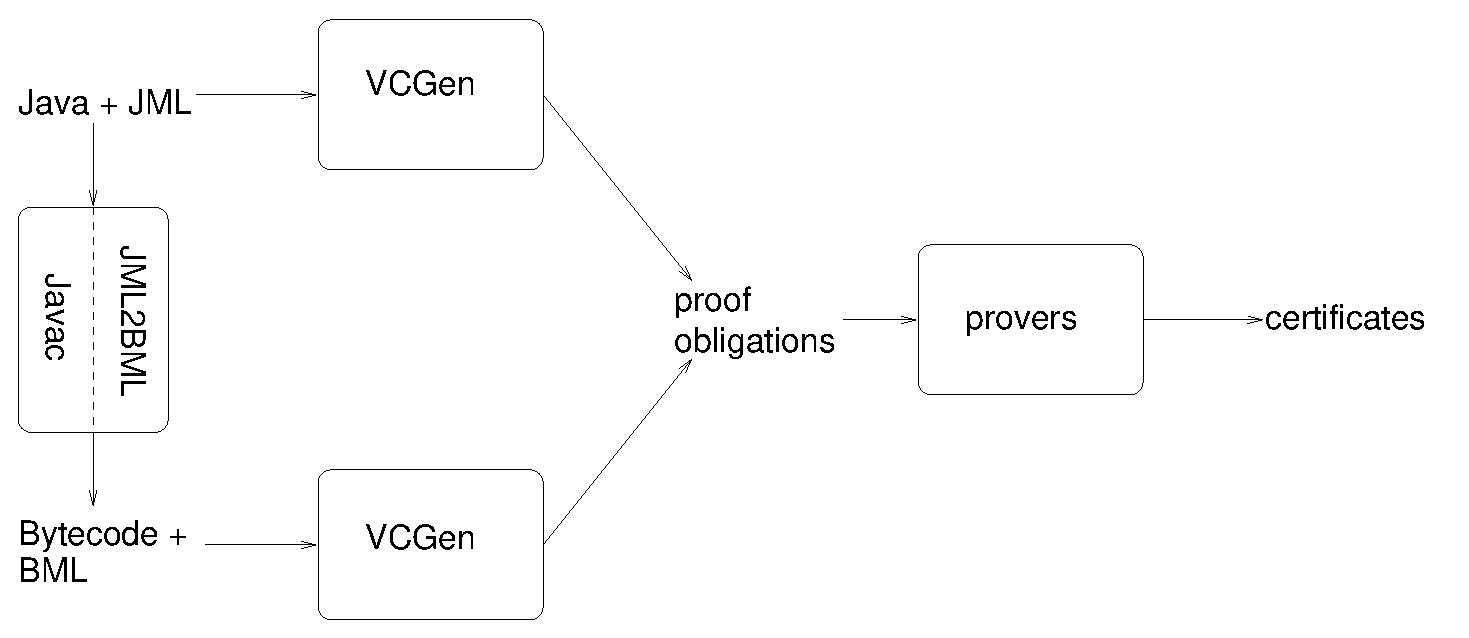
\includegraphics[width=\textwidth]{toolset.eps} 
\caption{Overview of \mobius tool set}\label{FigToolSet}
\end{figure}
As part of the \mobius project, we plan to develop a tool set that
supports both JML and BML. Figure~\ref{FigToolSet} outlines the
general architecture of this tool set. Thus, both Java/JML and
bytecode/BML can be used as input application. For both specification
languages, verification condition generators are used to generate
appropriate proof obligations that can be discharged with a theorem
prover (either automatic or interactive). To support the proof
carrying code platform, the provers will be instrumented to produce
certificates. In addition, source code applications annotated with JML
can be compiled into bytecode annotated with BML.

The development of the JML subcomponent of the tool set will be based
on experiences with ESC/Java~\cite{CokK04} and JACK~\cite{BurdyRL03}.
Several tools and algorithms (notably the compiler and the
verification condition generator) for BML have already been
implemented, see~\cite{BurdyP06}, but more work is needed to cover the
whole language. Moreover, to make the tool set usable in practice, we
will also need a tool to inspect and write directly BML
specifications, and a run-time checker for BML specifications. The
latter can be implemented by a code transformation, inserting explicit
run-time checks in the bytecode, or by extending the virtual machine
to take the user-specific attributes with specifications into account;

Our initial experiments with compilation of specifications has shown
that there exists indeed a correspondence between the proof
obligations generated at source and at bytecode level, modulo
differences in elimination of trivial goals, handling of arithmetic
expressions, and the naming convention of generated
variables. Moreover, when the proofs are done with the Coq prover,
different names are generated for hypotheses at source code and
bytecode level. It is future work to clean up the compilation, so
there is a one-to-one correspondence.




 

\subsection*{Related work}
The interest in specification and verification of bytecode
applications is quite recent, and not too much work has been done in
that direction. Several logics have been developed to reason about
bytecode, \emph{e.g.}~by Bannwart \& M\"uller~\cite{BannwartMueller05}
and within the MRG project~\cite{AspinallEtAl:TPHOLs2004}. However,
in this work, no attention is given to how one can conveniently write
understandable specifications for bytecode.

The development of BML is clearly inspired by the development of the
JML specification language~\cite{JMLReferenceManual05}. Both JML and
BML follow the Design by Contract principle introduced first in
Eiffel~\cite{Meyer97}. The Boogie project~\cite{BarnettCDJL05}
introduces in similarly the Design by Contract principles into the C\#
programming language, both at source code level and for CIL, the .NET
intermediate language.  The possibility to check a property at
run-time, using the \texttt{assert} construct, has been long 
adopted in the C programming language and recently also in Java (Java
1.5, see \cite[\S 14.10]{JLS}). 

Finally, we should mention the Extended Virtual Platform
project\footnote{See
\url{http://www.cs.usm.maine.edu/~mroyer/xvp/}.}. This project aims at
developing a framework that allows to compile JML annotations, to
allow run-time checking~\cite{AlagicXVP05}. However, in contrast to
our work, they do not intend to do static verification of bytecode
programs. Moreover, their platform takes JML-annotated source code
files as starting point, while with BML one is able to annotate
bytecode applications directly\footnote{Some security-critical
applications are written in bytecode directly, to avoid security
problems related with compilation. Thus, for such applications one
needs to be able to specify and verify them directly at this level.}.



\subsection*{Acknowledgements}
We thank Lennart Beringer and Olha Shkaravska for discussions about
the semantics of BML. 


\bibliographystyle{plain}
\bibliography{bibli,../specification,everest,crossrefs,strings}

\end{document}
